\documentclass[12pt,fleqn]{article}
\pagestyle {plain}
\usepackage {graphicx}
\usepackage {amsfonts}
\usepackage {setspace}
\usepackage {slashbox}
\usepackage {pict2e}
\usepackage {amsmath}
\usepackage {url}
\topmargin -.25 in \oddsidemargin .15 in \textwidth
6 in \textheight 8in


\title{Using an Ice Cream Cone to Gain Proficiency in Triple Integration}
%\author{Paul Isihara and Julia Lailler}
\author{}

\date{}


\begin{document}
\maketitle
\doublespacing
             Answer this problem within five minutes and you pass our proficiency check of triple integration:

\begin{quote}
\emph{Change the following integral in spherical coordinates
\begin{displaymath}
\int_{\theta=0}^{2\pi}\int_{\phi=0}^{\pi/4} \int_{\rho=0}^{\cos(\phi)} \rho^2\sin(\phi) \,d\rho\,d\phi\,d\theta
 \end{displaymath}
 {\flushleft to} cylindrical coordinates in $d\theta\,dr\,dz$ order.}
\end{quote}

Having failed a similar proficiency check posed by my junior co-author, we  unfold a few underlying ideas.    
    To begin, consider the volume $V$ situated above the cone $z=\sqrt{x^2+y^2}$ and below the sphere $x^2+y^2+z^2=1$ (Figure \ref{ic1}).   These bounding surfaces are easily expressed in cylindrical coordinates as $z=r$ (cone) and $z=\sqrt{1-r^2}$ (sphere). So is the disc in the xy plane ($0\le r\le1$) over which these surfaces are situated. The volume is also easy to describe in spherical coordinates ($0\le \phi\le \frac{\pi}{4}$, $0\le \rho \le 1$, $0\le\theta\le 2\pi$).  As a result, this ``ice cream cone" is simply represented in Cartesian, cylindrical, and spherical coordinates:
              \begin{figure*}[!htpb]
    \centering
        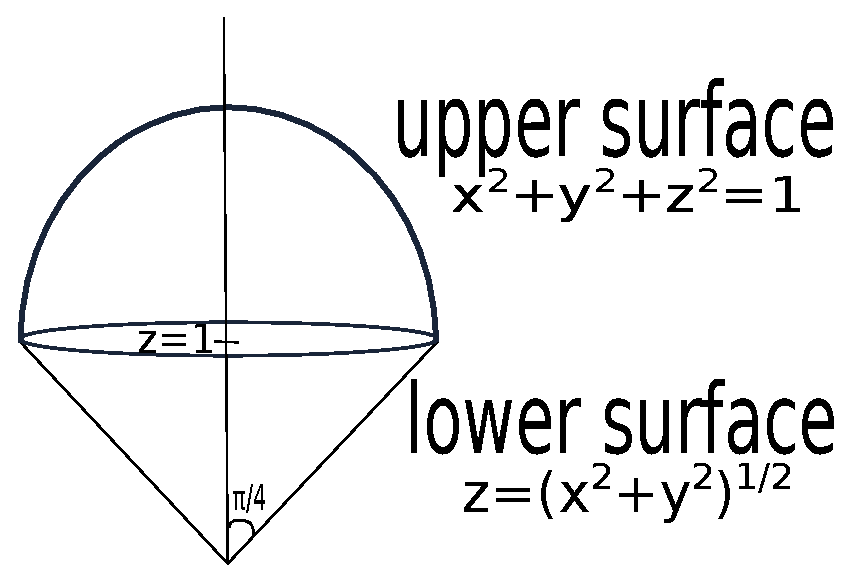
\includegraphics [width=2.25in, height=1.65in]{ic1.eps}
    \caption{Simple ice cream cone with volume $V$.}
    \label{ic1}
\end{figure*}
             
          
\begin{eqnarray*}
V &= &  \int_{x=-1}^{x=1} \int_{y=-\sqrt{1-x^2}}^{y=\sqrt{1-x^2}}\int_{z=\sqrt{x^2+y^2}}^{z=\sqrt{1-x^2-y^2}}\,dz\,dy\,dx  \hspace{.1in} \textup{(Cartesian),}\\
&=&\int_{\theta=0}^{2\pi}\int_{r=0}^{r=1} \int_{z=r}^{z=\sqrt{1-r^2}} r \,dz\,dr\,d\theta \hspace{.1in} \textup{(cylindrical),}\\
& = &\int_{\theta=0}^{2\pi}\int_{\phi=0}^{\pi/4} \int_{\rho=0}^{1} \rho^2\sin(\phi) \,d\rho\,d\phi\,d\theta \hspace{.1in} \textup{(spherical)}.
\end{eqnarray*}


To check proficiency, we need a little harder ice cream cone. Following  \cite{S}, we change the capping surface  to $x^2+y^2+z^2=z$ (see Figure \ref{ic3}).  


\begin{figure*}[h]
    \centering
        \includegraphics [width=3.25in, height=1.5in]{ic3.eps}
    \caption{Volume $V_1$ has a new capping surface representable in both cylindrical and spherical coordinates.}
    \label{ic3}
\end{figure*}

{\flushleft By} completing squares, we know that the capping surface  is part of a hemisphere centered at (0,0,1/2) with radius 1/2. 
The new volume $V_1$ is situated above the cone  $z=\sqrt{x^2+y^2}=r$ and below the sphere $z=\frac {1}{2}+\sqrt{\frac{1}{4}-x^2-y^2}=\frac{1}{2}+\sqrt{\frac{1}{4}-r^2}$ with both surfaces situated over the disk $x^2+y^2 \le 1/4$ (equivalently $r\le\frac{1}{2}$) in the $xy$ plane.
In spherical, since $x^2+y^2+z^2=\rho^2$ and $z=\rho\cos(\phi)$, the new capping surface is $\rho=\cos(\phi)$. Hence, the new volume $V_1$ is still easily representable by triple integrals in all three coordinate systems:

\begin{eqnarray}
V_1&=& \int_{x=-1/2}^{x=1/2} \int_{y=-\sqrt{\frac{1}{4}-x^2}}^{\sqrt{\frac{1}{4}-x^2}}\int_{z=\sqrt{x^2+y^2}}^{\frac {1}{2}+\sqrt{\frac{1}{4}-x^2-y^2}}\,dz\,dy\,dx \hspace{.1in} \textup{(Cartesian),} \nonumber\\
&=&\int_{\theta=0}^{2\pi}\int_{r=0}^{r=1/2} \int_{z=r}^{z=\frac {1}{2}+\sqrt{\frac{1}{4}-r^2}} r \,dz\,dr\,d\theta \hspace{.1in} \textup{(cylindrical),} \nonumber\\
 &=&\int_{\theta=0}^{2\pi}\int_{\phi=0}^{\pi/4} \int_{\rho=0}^{\cos(\phi)} \rho^2\sin(\phi) \,d\rho\,d\phi\,d\theta \hspace{.1in} \textup{(spherical). \label{eqn1}}
\end{eqnarray}

In addition to thinking of $V_1$ as a volume between two surfaces or as a portion of a sphere, a third conceptualization involves cross-sectional disks centered on the $z$-axis (Figure \ref{ic4}). 

\begin{figure*}[h]
    \centering
        \includegraphics [width=2.5in, height=1.25in]{ic4.eps}
    \caption{Volume $V_1$ by cross sectional disks.}
    \label{ic4}
\end{figure*}

{\flushleft In} this case we again use cylindrical coordinates, but to account for differences in radii of the discs, we must divide the volume into two parts, the conical base  and the spherical cap:
\begin{eqnarray}
V_1 & = & \int_{z=0}^{z=.5}[\int_{r=0}^{r=z}\int_{\theta=0}^{\theta=2\pi} r\,d\theta\,dr]\,dz \hspace{.1in} \textup{(cone)}\nonumber\\
&& + \int_{z=.5}^{z=1}[\int_{r=0}^{r=[\sqrt{.25-(z-.5)^2}]^{1/2}}\int_{\theta=0}^{\theta=2\pi} r\,d\theta\,dr]\,dz \hspace{.1in} \textup{(cap)}.\label{eqn2}
\end{eqnarray}


{\flushleft Our} proficiency check is to show (\ref{eqn1}) $\Rightarrow$ (\ref{eqn2}). 





\begin{thebibliography}{5}

\bibitem{S} J. Stewart,  \emph{Calculus, Early Transcendentals (8E)}. Cengage Learning, Boston, 2016.

\end{thebibliography}

\end{document}
